%%body for test 1

\ques{15}
Consider the following {\bf MINIMIZING}, canonical form linear program, labeled (P):
\vspace{-2mm}

\begin{equation}
  \label{eq:1}
  \tag{P}
  \begin{array}{lll}
    \min & 3 x_1 \phantom{+  x_2} -  x_3 \phantom{+ 5 x_4} \\
    \mbox{s.t.} & x_1 + x_2 + x_3  + x_4 & = 4 \\[1mm]
    & -2 x_1 + x_2 - x_3  & = 1 \\
    & \phantom{-5 x_1} 3 x_2 + x_3 + x_4 &  = 9 \\
    & x_1, x_2, x_3, x_4 \geq 0 &
  \end{array}
\end{equation}



\begin{parts}
\pts{3} Because (P) is in canonical form, it is in the form minimize $\mathbf{c}^T \mathbf{x} $ such that $A\mathbf{x} = \mathbf{b}$ and $\mathbf{x} \geq \mathbf{0}$.  Find the matrix $A$ and the vectors $\mathbf{b}$, and $\mathbf{c}$. 


\vspace{6cm}

\pts{2} A Basic Feasible Solution to (P) will have \underline{ \ \ \ \ \ \ \ } basic variables and \underline{ \ \ \ \ \ \ \ } nonbasic variables.


\vspace{1.5cm}


\pts{4} Given the feasible direction $d^{x_3} = [-2/3, -1/3, 1, 0]^T$, determine whether or not it is an improving direction.  Based on your answer about whether the direction is improving, state whether the simplex algorithm would continue or terminate at this point.  {\bf Briefly} explain your answer for full credit.  You may find it helpful to recall that $\bar c_k = c^T d^k = c_k + \sum_{i \in \mathcal{B}} c_i d_i^k$.

\vfill
\newpage
\noindent \emph{Problem 1 continued.}


\pts{3} If the initial solution is $x^0 = [1,3,0,0]^T$, and the simplex direction is $d^{x_3} = [-2/3, -1/3, 1, 0]^T$ determine the maximum step size, $\lambda$.  Based on your answer about $\lambda$, which variable will leave the basis and become nonbasic? \emph{You may find it helpful to recall the ratio test: $\lambda = \min \left\{ \frac{x_j}{-d_j^k}:d_j^k < 0 \right\}$, or you may choose to find $\lambda$ without using the ratio test.} 



\vfill

\pts{3} If the initial solution is $x^0 = [1,3,0,0]^T$, use your answer from part (d) above to compute the new solution generated by this iteration of the Simplex Method.  If you were not able to answer part (d), use $\lambda = 3$.

\vfill

\end{parts}

\newpage

%%formulation given to answer about
\ques{25} The directed network shown below illustrates the supply chain for a small beverage company, NEHI. Node 1 represents a factory, nodes 2 and 3 are warehouses, and node 4 is a retail store. NEHI can ship crates of RC cola along any arc. The number $c_{ij}$ on the arc $(i,j)$ represents the cost per crate to ship from node $i$ to node $j$. Below, we show the start of a model whose purpose is to minimize shipping costs while meeting demand constraints. 

\begin{center}
        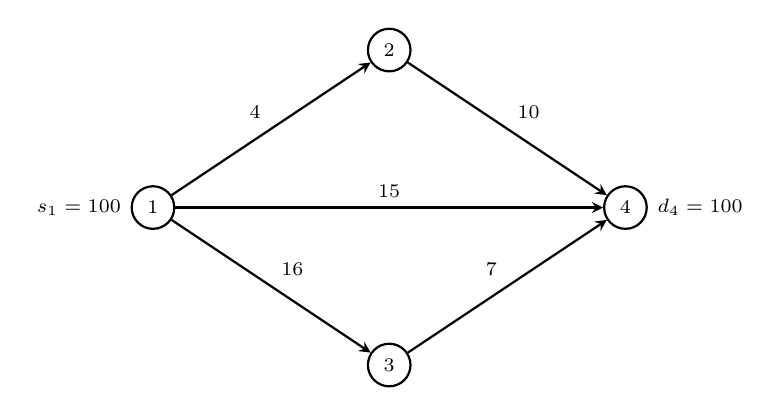
\begin{tikzpicture}
          [font=\scriptsize,
          node/.style={shape=circle,draw=black,fill=white!20, text=black,minimum width=0.5cm,thick},
          arc/.style={->,>=stealth,thick},
          edge/.style={thick}]
          
            \node (1) [node] at (0,0) [label = left:{$s_1 = 100$}] {1};
            \node (2) [node] at (3,2)  {2};
            \node (3) [node] at (3,-2) {3};
            \node (4) [node] at (6,0) [label = right:{$d_4 = 100$}] {4};
 
          \coordinate (A2) at (2.8,1.75);
          \coordinate (A3) at (2.8,-1.75);
          \coordinate (B2) at (3.2,1.75);
          \coordinate (B3) at (3.2,-1.75);
          
          
          \draw [arc] (1) to node [auto] {4} (2);
            \draw [arc] (1) to node [auto] {16} (3);
            %\draw [arc] (A2) to node [left] {3} (A3);
            %\draw [arc] (B3) to node [right] {5} (B2);
            \draw [arc] (2) to node [auto] {10} (4);
            \draw [arc] (3) to node [auto] {7} (4);
            \draw [arc] (1) to node [auto] {15} (4);

        \end{tikzpicture}
\end{center}

%\begin{picture}(77,55)(0,-55)
%\node[NLangle=0.0](n1)(16.0,-32.0){1}
%\node[NLangle=0.0](n2)(90.0,-12.0){2}
%\node[NLangle=0.0](n3)(90.0,-52.0){3}
%\node[NLangle=0.0](n4)(154.0,-32.0){4}
%\drawedge[ELdist=2.0](n1,n2){3}
%\drawedge[ELdist=-2.0](n1,n3){15}
%\drawedge[ELdist=6.0](n2,n3){2}
%\drawedge[ELdist=6.0](n3,n2){4}
%\drawedge[ELdist=2.0](n2,n4){9}
%\drawedge[ELdist=-2.0](n3,n4){6}
%\end{picture}



\noindent\underline{Sets}
\begin{tabbing}
\hspace{.5cm} \= $N$ \hspace{2.5cm} \= network nodes ($N=\{1,2,3,4\}$) \\
\> $E$ \>  network edges $(i,j)$ directed from node $i$ to node $j$ \\

\noindent\underline{Data}\\% [units]\\
\> {\it C}$_{ij}$ \> shipping cost in dollars/case over edge $(i,j)$ \\
\> $S_1=100$ \> supply at node 1 \\
\> $D_4=100$ \> demand at node 4 \\
%\> {\it capacity}$_2 = 60$ \> upper bound on warehouse 2 in cases \\
%\> {\it capacity}$_3 = 40$ \> upper bound on warehouse 3 in cases \\

\noindent\underline{Decision Variables}\\% [units]\\
\> {\it x}$_{ij}$ \> Number of cases shipped on arc $(i,j)$  \\
\end{tabbing}

\newpage
\noindent \emph{Problem 2 continued.}

\begin{parts}
\pts{6}
If the factory at node 1 has a supply of 100 cases, nodes 2 and 3 are warehouses with no supply or demand, and node 4 is a store with a demand of 100 cases, write the constraints that ensure that the flows $x_{ij}$ are valid in this context.   Use only VARIABLES and NUMBERS.  (No sets or summations.)
\vfill
%\vspace{0.75cm}
%
%
%\pts{6} Write the balance of flow constraint for node 4.
%
%\vspace{2.75cm}

\pts{5} The warehouses at nodes 2 and 3 can only be used if a fixed charge is paid to open the warehouse:  $F_1 = \$300$ for node 2 and $F_2 = \$200$ for node 3. Write an objective function that minimizes the total cost of shipping and the fixed charges associated with opening one (or both) of the warehouses (i) using only VARIABLES and NUMBERS (4 points)  (ii) using SET notation (1 points). \emph{Be sure to define any items you use in your objective function that are not already given above.}

\vfill 

\newpage
\noindent \emph{Problem 2 continued.}

\pts{4} Write the two constraints that ensure that we are charged for any warehouse that is used. % Be sure to define any items you use in your constraints that are not already given above.  
Use only VARIABLES and NUMBERS. Be sure to define any items you use in your constraints that are not already given above.

\vfill

\pts{3} The brothers that run NEHI have just learned of a new, unusual, shipping requirement. If they send more than 20 cases from the factory to the warehouse at node 2 then they must also send at least 30 cases from the factory to the warehouse at node 3. Introduce constraints that impose this condition. Be sure to define any items you use in your constraints that are not already given above.

\vfill


\end{parts}
\newpage

\ques{20}
As a newly commissioned 2nd Lt you have been tasked with connecting 6 forward operating bases (located at nodes 1 through 6) at minimal cost.  Connecting a base to another base has a cost, and each base must have a ``path'' of wiring to every other base. However, not every base can be wired directly to every other base.  Your boss, Capt May B. Wright has
determined that the locations and possible connections form the following network, with costs
($c_{ij}$ in thousands of dollars) listed next to the arcs (you may assume he is correct in his drawing). He has denoted the network $\cG = (\cV, \cE)$:

\begin{center}
        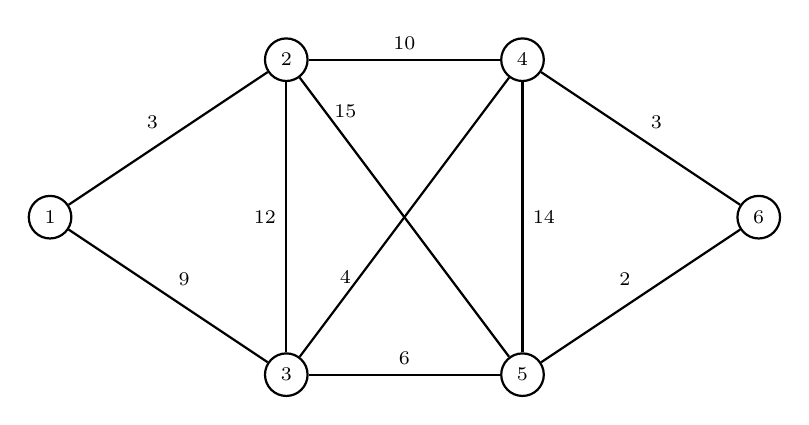
\begin{tikzpicture}
          [font=\scriptsize,
          node/.style={shape=circle,draw=black,fill=white!20, text=black,minimum width=0.5cm,thick},
          arc/.style={->,>=stealth,thick},
          edge/.style={thick}]
          
            \node (1) [node] at (0,0) {1};
            \node (2) [node] at (3,2) {2};
            \node (3) [node] at (3,-2) {3};
            \node (4) [node] at (6,2) {4};
            \node (5) [node] at (6,-2) {5};
            \node (6) [node] at (9,0) {6};
         
          
          \draw [edge] (1) to node [auto] {3} (2);
          \draw [edge] (1) to node [auto] {9} (3);
          \draw [edge] (2) to node [left] {12} (3);
          \draw [edge] (2) to node [auto] {10} (4);
          \draw [edge] (3) to node [auto] {6} (5);
          \draw [edge] (4) to node [auto] {14} (5);
          \draw [edge] (4) to node [auto] {3} (6);
          \draw [edge] (5) to node [auto] {2} (6);
          \draw [edge] (2) to node [label={[shift={(-0.75,1.0)}]15}] {} (5);
          \draw [edge] (3) to node [label={[shift={(-0.75,-1.1)}]4}] {} (4);

        \end{tikzpicture}
\end{center}

Thus, you are trying to determine a minimum spanning tree on
the given network. We denote the edge between two nodes $i$ and $j$ by the pair $(i,j)$ with $i<j$ and define the binary variables $X_{ij}$ to be one when the edge $(i,j)$ is in the minimum spanning tree and zero otherwise. Capt Wright started formulating the integer program below, labeled \eqref{eq:mst}:
\begin{equation}
  \label{eq:mst}
  \tag{MST}
  \begin{array}{llll}
    \min & \Sum_{(i,j) \in \cE} c_{ij} X_{ij} & & \\
    \mbox{s.t.} & \Sum_{\{j | (i,j) \in \cE\}} X_{ij} + 
    \Sum_{\{j |(j,i) \in \cE\}} X_{ji} \geq {?}, & \forall i \in \cV &
    \mbox{(a)} \\[4mm]
    & \Sum_{(i,j) \in \cE} X_{ij} = |\cV| - 1 & & \mbox{(b)} \\[4mm]
    %& \Sum_{(i,j) \in \cE | i,j \in U} X_{ij} \leq |U| - 1 & \forall U
    %\subset \cV, 3 \leq |U| \leq |V| - 1 & \mbox{(b)} \\[4mm]
    & X_{ij} \in \{0,1\} & \forall (i,j) \in \cE. &
  \end{array}
\end{equation}

\newpage
\noindent \emph{Problem 3 continued.}

\begin{parts}
  
\pts{4} Capt Wright wasn't sure what should go on the right hand side of the inequality for constraint (a) in \eqref{eq:mst}.  Specify what should replace the ? on the right hand side of the inequality.  For full credit you MUST also explain in words what this constraint is enforcing. 

\vfill


\pts{6} Write down the associated constraint of type (b) from \eqref{eq:mst} using only VARIABLES and NUMBERS.  For full credit you MUST explain in words what this constraint is enforcing.

\vfill

\newpage
\noindent \emph{Problem 3 continued.}


\pts{6} Capt Wright solves \eqref{eq:mst} and obtains the solution $X_{12} = X_{35} = X_{46} = X_{56} = X_{34} = 1$, all other $X_{ij} = 0$.  Graphically illustrate (using nodes and edges) what this solution represents. 

\vspace{2cm}
\vfill

\pts{4} Does the solution in part c above represent a minimum cost spanning tree?  If your answer is \mbox{\bf{YES}}, then give the value of the objective function for this solution.  If your answer is \mbox{\bf{NO}}, use the variables $X_{ij}$ to write a constraint that you would add to \eqref{eq:mst} before you attempt to solve the model again.


\vfill

%\pts{4} CDR Wright insists that the \mbox{\bf{SINGLE}} constraint you wrote in part (c) \mbox{\bf{GUARANTEES}} that the solver will return a minimum spanning tree once the model is solved again.  Explain in complete sentences why you agree or disagree with CDR Wright.

%\vfill

\end{parts}

% \newpage

% %%true/false/multiple choice
% \ques{10} True or False. No justification needed.
% \begin{itemize}
%   \tfl If the simplex method returns an optimal solution for a linear
%   program in canonical form with $m$ constraints and $n$ variables,
%   then the solution could have more than $n-m$ variables set to zero.

%   \tfl All feasible linear programs that are not unbounded have extreme point optimal solutions.

%   \tfl A d
% \end{itemize}
%%LP questions 20-30%




\newpage

%%some graph problems?

%%bonus question

%\bques{10}
%Recall that an undirected graph, $\cG = (\cV,\cE)$, is a tree if $\cG$ is connected (there is a path between every pair of nodes), and has no cycles. A leaf is a node in a tree with exactly one arc adjacent to it. Prove that any tree has at least two leaves, assuming that the number of nodes, $n$, is greater than or equal to two. 

% Start a path at an arbitrary node, walking to any neighbor that hasn't been visited before.  After at most $n$ steps, we must reach a node $v$ where there are no untraversed neighbors.  Therefore, $v$ must have only one neighbor and is a leaf, otherwise there is a cycle and the graph is not a tree.  We can then traverse a path starting at $v$, and the node where the path stops must be a second leaf.